
%(BEGIN_QUESTION)
% Copyright 2015, Tony R. Kuphaldt, released under the Creative Commons Attribution License (v 1.0)
% This means you may do almost anything with this work of mine, so long as you give me proper credit

This valve positioner system, shown in the fully-closed position, has a problem.  When placed into service, the valve remains at 100\% (full open) for {\it any} applied control signal value:

$$\includegraphics[width=15.5cm]{i01361x01.eps}$$

Looking at the gauges, you notice the supply gauge reads 95 PSI, the control signal gauge reads 4.3 PSI, and the output gauge reads 88 PSI.

Identify the likelihood of each specified fault for this valve positioner.  Consider each fault one at a time (i.e. no coincidental faults), determining whether or not each fault could independently account for {\it all} measurements and symptoms.

% No blank lines allowed between lines of an \halign structure!
% I use comments (%) instead, so that TeX doesn't choke.

$$\vbox{\offinterlineskip
\halign{\strut
\vrule \quad\hfil # \ \hfil & 
\vrule \quad\hfil # \ \hfil & 
\vrule \quad\hfil # \ \hfil \vrule \cr
\noalign{\hrule}
%
% First row
{\bf Fault} & {\bf Possible} & {\bf Impossible} \cr
%
\noalign{\hrule}
%
% Another row
Plugged restriction &  &  \cr
%
\noalign{\hrule}
%
% Another row
Plugged nozzle &  &  \cr
%
\noalign{\hrule}
%
% Another row
Broken spring &  &  \cr
%
\noalign{\hrule}
%
% Another row
Leak in bellows &  &  \cr
%
\noalign{\hrule}
%
% Another row
Leak in actuator diaphragm &  &  \cr
%
\noalign{\hrule}
%
% Another row
Air supply failure &  &  \cr
%
\noalign{\hrule}
} % End of \halign 
}$$ % End of \vbox

Finally, identify the {\it next} diagnostic test or measurement you would make on this system.  Explain how the result(s) of this next test or measurement help further identify the location and/or nature of the fault.

\underbar{file i01361}
%(END_QUESTION)





%(BEGIN_ANSWER)

A good diagnostic test here would be to pull the flapper away from the nozzle with your finger to see if the valve actuator returns to the ``closed'' (0\%) position.
 
%(END_ANSWER)





%(BEGIN_NOTES)

% No blank lines allowed between lines of an \halign structure!
% I use comments (%) instead, so that TeX doesn't choke.

$$\vbox{\offinterlineskip
\halign{\strut
\vrule \quad\hfil # \ \hfil & 
\vrule \quad\hfil # \ \hfil & 
\vrule \quad\hfil # \ \hfil \vrule \cr
\noalign{\hrule}
%
% First row
{\bf Fault} & {\bf Possible} & {\bf Impossible} \cr
%
\noalign{\hrule}
%
% Another row
Plugged restriction &  & $\surd$ \cr
%
\noalign{\hrule}
%
% Another row
Plugged nozzle & $\surd$ &  \cr
%
\noalign{\hrule}
%
% Another row
Broken spring & $\surd$ &  \cr
%
\noalign{\hrule}
%
% Another row
Leak in bellows &  & $\surd$ \cr
%
\noalign{\hrule}
%
% Another row
Leak in actuator diaphragm &  & $\surd$ \cr
%
\noalign{\hrule}
%
% Another row
Air supply failure &  & $\surd$ \cr
%
\noalign{\hrule}
} % End of \halign 
}$$ % End of \vbox

\vskip 20pt \vbox{\hrule \hbox{\strut \vrule{} {\bf Virtual Troubleshooting} \vrule} \hrule}

This question is a good candidate for a ``Virtual Troubleshooting'' exercise.  Presenting the diagram to students, you first imagine in your own mind a particular fault in the system.  Then, you present one or more symptoms of that fault (something noticeable by an operator or other user of the system).  Students then propose various diagnostic tests to perform on this system to identify the nature and location of the fault, as though they were technicians trying to troubleshoot the problem.  Your job is to tell them what the result(s) would be for each of the proposed diagnostic tests, documenting those results where all the students can see.

During and after the exercise, it is good to ask students follow-up questions such as:

\begin{itemize}
\item{} What does the result of the last diagnostic test tell you about the fault?
\item{} Suppose the results of the last diagnostic test were different.  What then would that result tell you about the fault?
\item{} Is the last diagnostic test the best one we could do?
\item{} What would be the ideal order of tests, to diagnose the problem in as few steps as possible?
\end{itemize}



\vfil \eject

\noindent
{\bf Summary Quiz:}

Identify the effect(s) of the nozzle plugging with debris in this valve positioner mechanism:

$$\includegraphics[width=15.5cm]{i01361x01.eps}$$

\begin{itemize}
\item{} The control valve will move to the full-closed position 
\vskip 5pt 
\item{} The spring will stretch until it breaks
\vskip 5pt 
\item{} The control valve will move to the full-open position
\vskip 5pt 
\item{} The control valve will hold its last position firmly
\vskip 5pt 
\item{} The bellows will fully inflate
\vskip 5pt 
\item{} The control valve will oscillate back and forth 
\end{itemize}

%INDEX% Final Control Elements, valve: positioner (troubleshooting) 

%(END_NOTES)


